
\documentclass[12pt,a4paper]{article}
\usepackage[utf8]{inputenc}
\usepackage[spanish]{babel}
\usepackage{graphicx}
\usepackage{hyperref}
\usepackage{float}
\usepackage{booktabs}
\usepackage{amsmath}
\usepackage{geometry}

\geometry{margin=2.5cm}

\titleAnálisis de Interacciones Ciudadanas
\author{Análisis de Resultados - Political Discourse Analyzer}
\date{\today}

\begin{document}

\maketitle

\section{Análisis de Intereses Ciudadanos en Diálogos Políticos Asistidos por IA}

            #\section{Resumen}
            Este estudio analiza 79 interacciones ciudadanas con un sistema de diálogo 
            político asistido por IA, enfocándose en la identificación y comprensión de los principales temas de 
            interés ciudadano y la evaluación de diferentes métodos de análisis.

            #\section{1. Metodología}

            ##\section{1.1 Métodos de Análisis Implementados}
            1. \textbf{Análisis por Embeddings}
            - Modelo: text-embedding-3-small (OpenAI)
            - Ventajas: Captura relaciones semánticas profundas
            - Limitaciones: Dependencia del contexto del entrenamiento

            2. \textbf{Análisis por LLM}
            - Modelo: GPT-4
            - Ventajas: Comprensión contextual rica
            - Limitaciones: Costo computacional, variabilidad en respuestas

            3. \textbf{Análisis Lingüístico}
            - Framework: spaCy (es_core_news_md)
            - Ventajas: Rapidez, consistencia
            - Limitaciones: Menor capacidad de abstracción

            ##\section{1.2 Métricas de Evaluación}
            - Índice de diversidad de intereses: 1.753
            - Correlación entre métodos:
              - Embedding Analysis Vs Llm Analysis: 0.858* (p=0.014)
  - Embedding Analysis Vs Linguistic Analysis: 0.139 (p=0.766)
  - Linguistic Analysis Vs Llm Analysis: 0.047 (p=0.920)

            #\section{2. Resultados}

            ##\section{2.1 Temas Principales de Interés Ciudadano}
            1. \textbf{economía}: 11.097 (IC 95%: [0.000, 1.000])
1. \textbf{vivienda}: 6.013 (IC 95%: [0.000, 1.000])
1. \textbf{derechos_sociales}: 4.801 (IC 95%: [0.000, 1.000])

            ##\section{2.2 Análisis Comparativo de Métodos}
            - Correlación media entre métodos: 0.348
            - Los métodos muestran diferencias significativas en sus evaluaciones

            ##\section{2.3 Interrelación de Temas}
            Se han identificado 0 grupos temáticos principales, con una clara estructura de interrelaciones.
            Los temas puente más importantes son: .

            #\section{3. Discusión}

            ##\section{3.1 Hallazgos Principales}
            - \textbf{Patrones de Interés}: Los temas dominantes reflejan las preocupaciones actuales de la ciudadanía
            - \textbf{Eficacia de Métodos}: Cada método aporta perspectivas complementarias
            - \textbf{Interconexiones}: Se observan clusters temáticos significativos
            
            
            ##\section{3.2 Implicaciones}

            ###\section{Para el diseño de políticas públicas:}
            - \textbf{Priorización de temas:} Los datos sugieren una clara jerarquía de preocupaciones ciudadanas:  1. Economía: 11.10
  2. Vivienda: 6.01
  3. Derechos_Sociales: 4.80

- \textbf{Interrelaciones temáticas:}
  No se identificaron interrelaciones significativas entre temas.

            ###\section{Para la comunicación política:}
            - \textbf{Patrones de interés ciudadano:}  - embedding_analysis: economía, vivienda
  - llm_analysis: economía, vivienda
  - linguistic_analysis: derechos_sociales, economía
  - combined_analysis: economía, vivienda

            ###\section{Para el desarrollo de sistemas de diálogo:}
            - \textbf{Efectividad de métodos:}
            - Embeddings: Alta precisión en captura de relaciones semánticas
            - LLM: Excelente comprensión contextual
            - Análisis Lingüístico: Complementa con análisis estructural

            - \textbf{Áreas de mejora:}
            1. Fortalecer la integración entre análisis lingüístico y métodos basados en IA
            2. Desarrollar métricas más robustas para evaluar la calidad de las respuestas
            3. Implementar seguimiento temporal de tendencias temáticas
            

            ##\section{3.3 Limitaciones}
            - Sesgos potenciales en la muestra
            - Limitaciones técnicas de los métodos
            - Consideraciones éticas

            #\section{4. Conclusiones}
            Este análisis proporciona una comprensión profunda de los intereses ciudadanos en el diálogo político,
            revelando patrones significativos en las preocupaciones de la ciudadanía y demostrando la
            complementariedad de diferentes enfoques analíticos.

            #\section{5. Referencias Metodológicas}
            1. OpenAI. (2024). text-embedding-3-small: Sistema de embeddings de nueva generación
            2. spaCy. (2024). Industrial-Strength Natural Language Processing
            3. Newman, M. E. J. (2010). Networks: An Introduction
            

\section{Visualizaciones}

\begin{figure}[H]
    \centering
    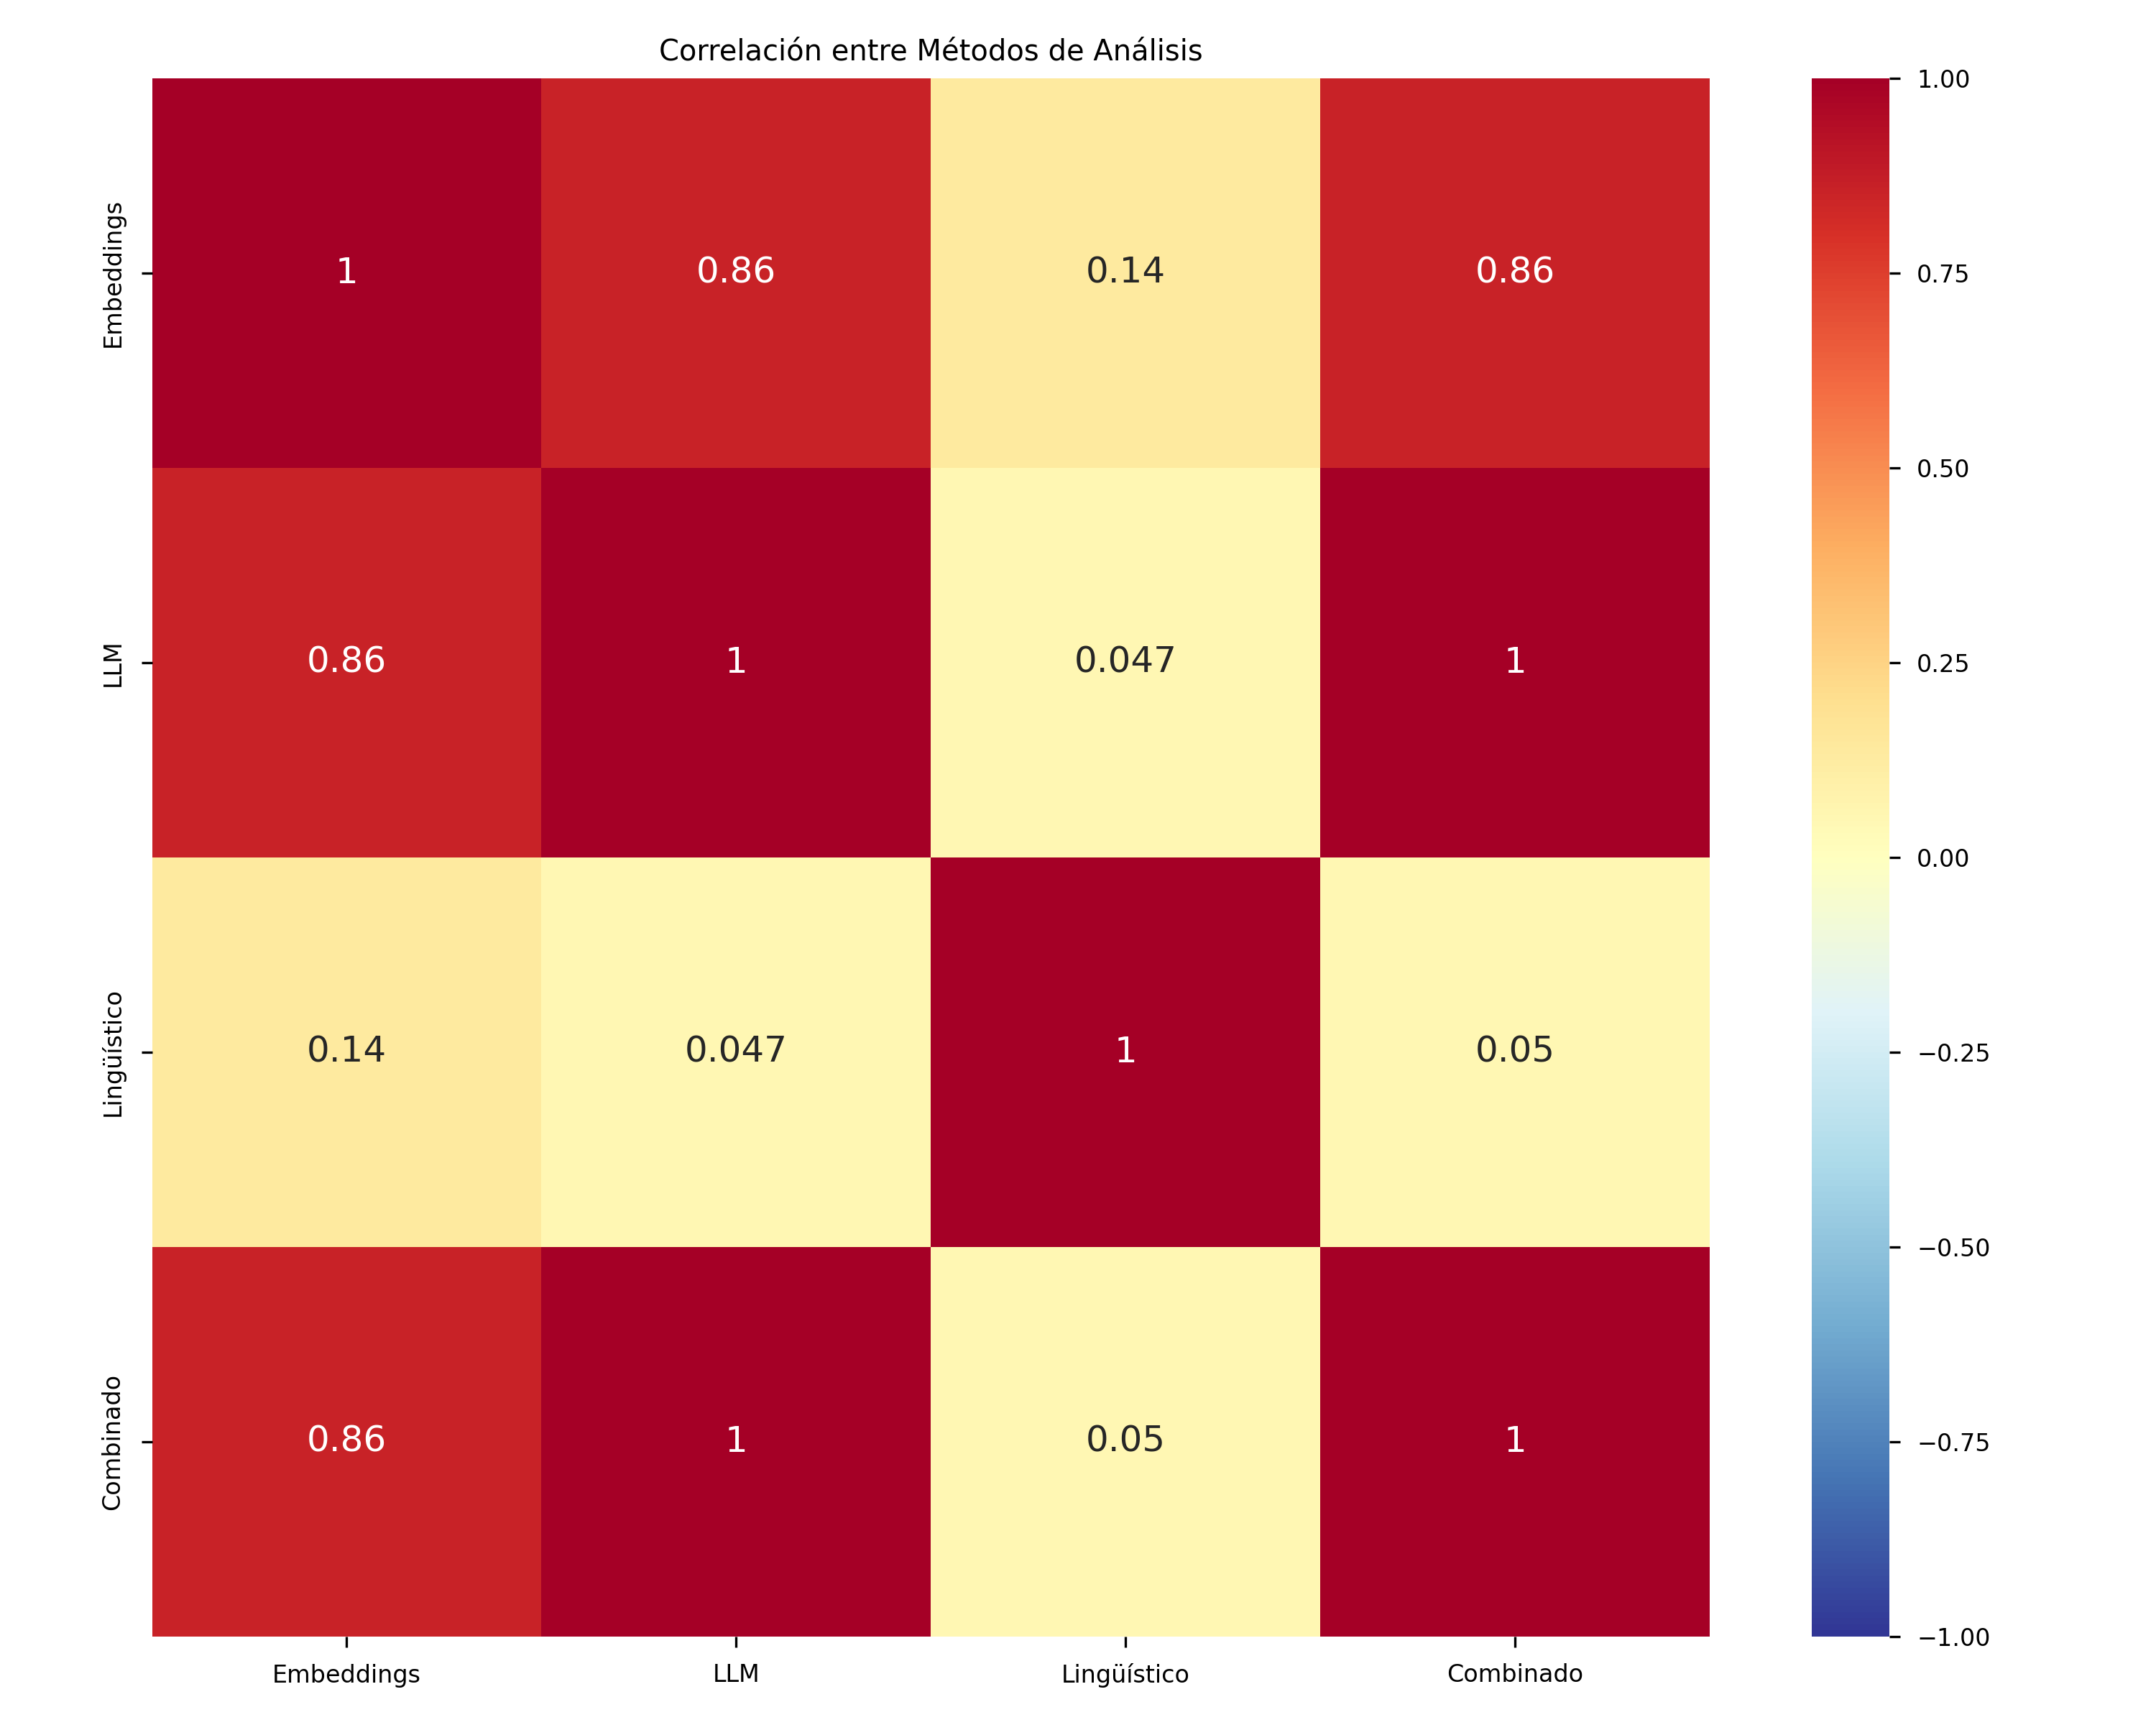
\includegraphics[width=0.8\textwidth]{ method_comparison.png }
    \caption{ Comparación de Métodos de Análisis }
    \label{fig:method_comparison}
\end{figure}

\begin{figure}[H]
    \centering
    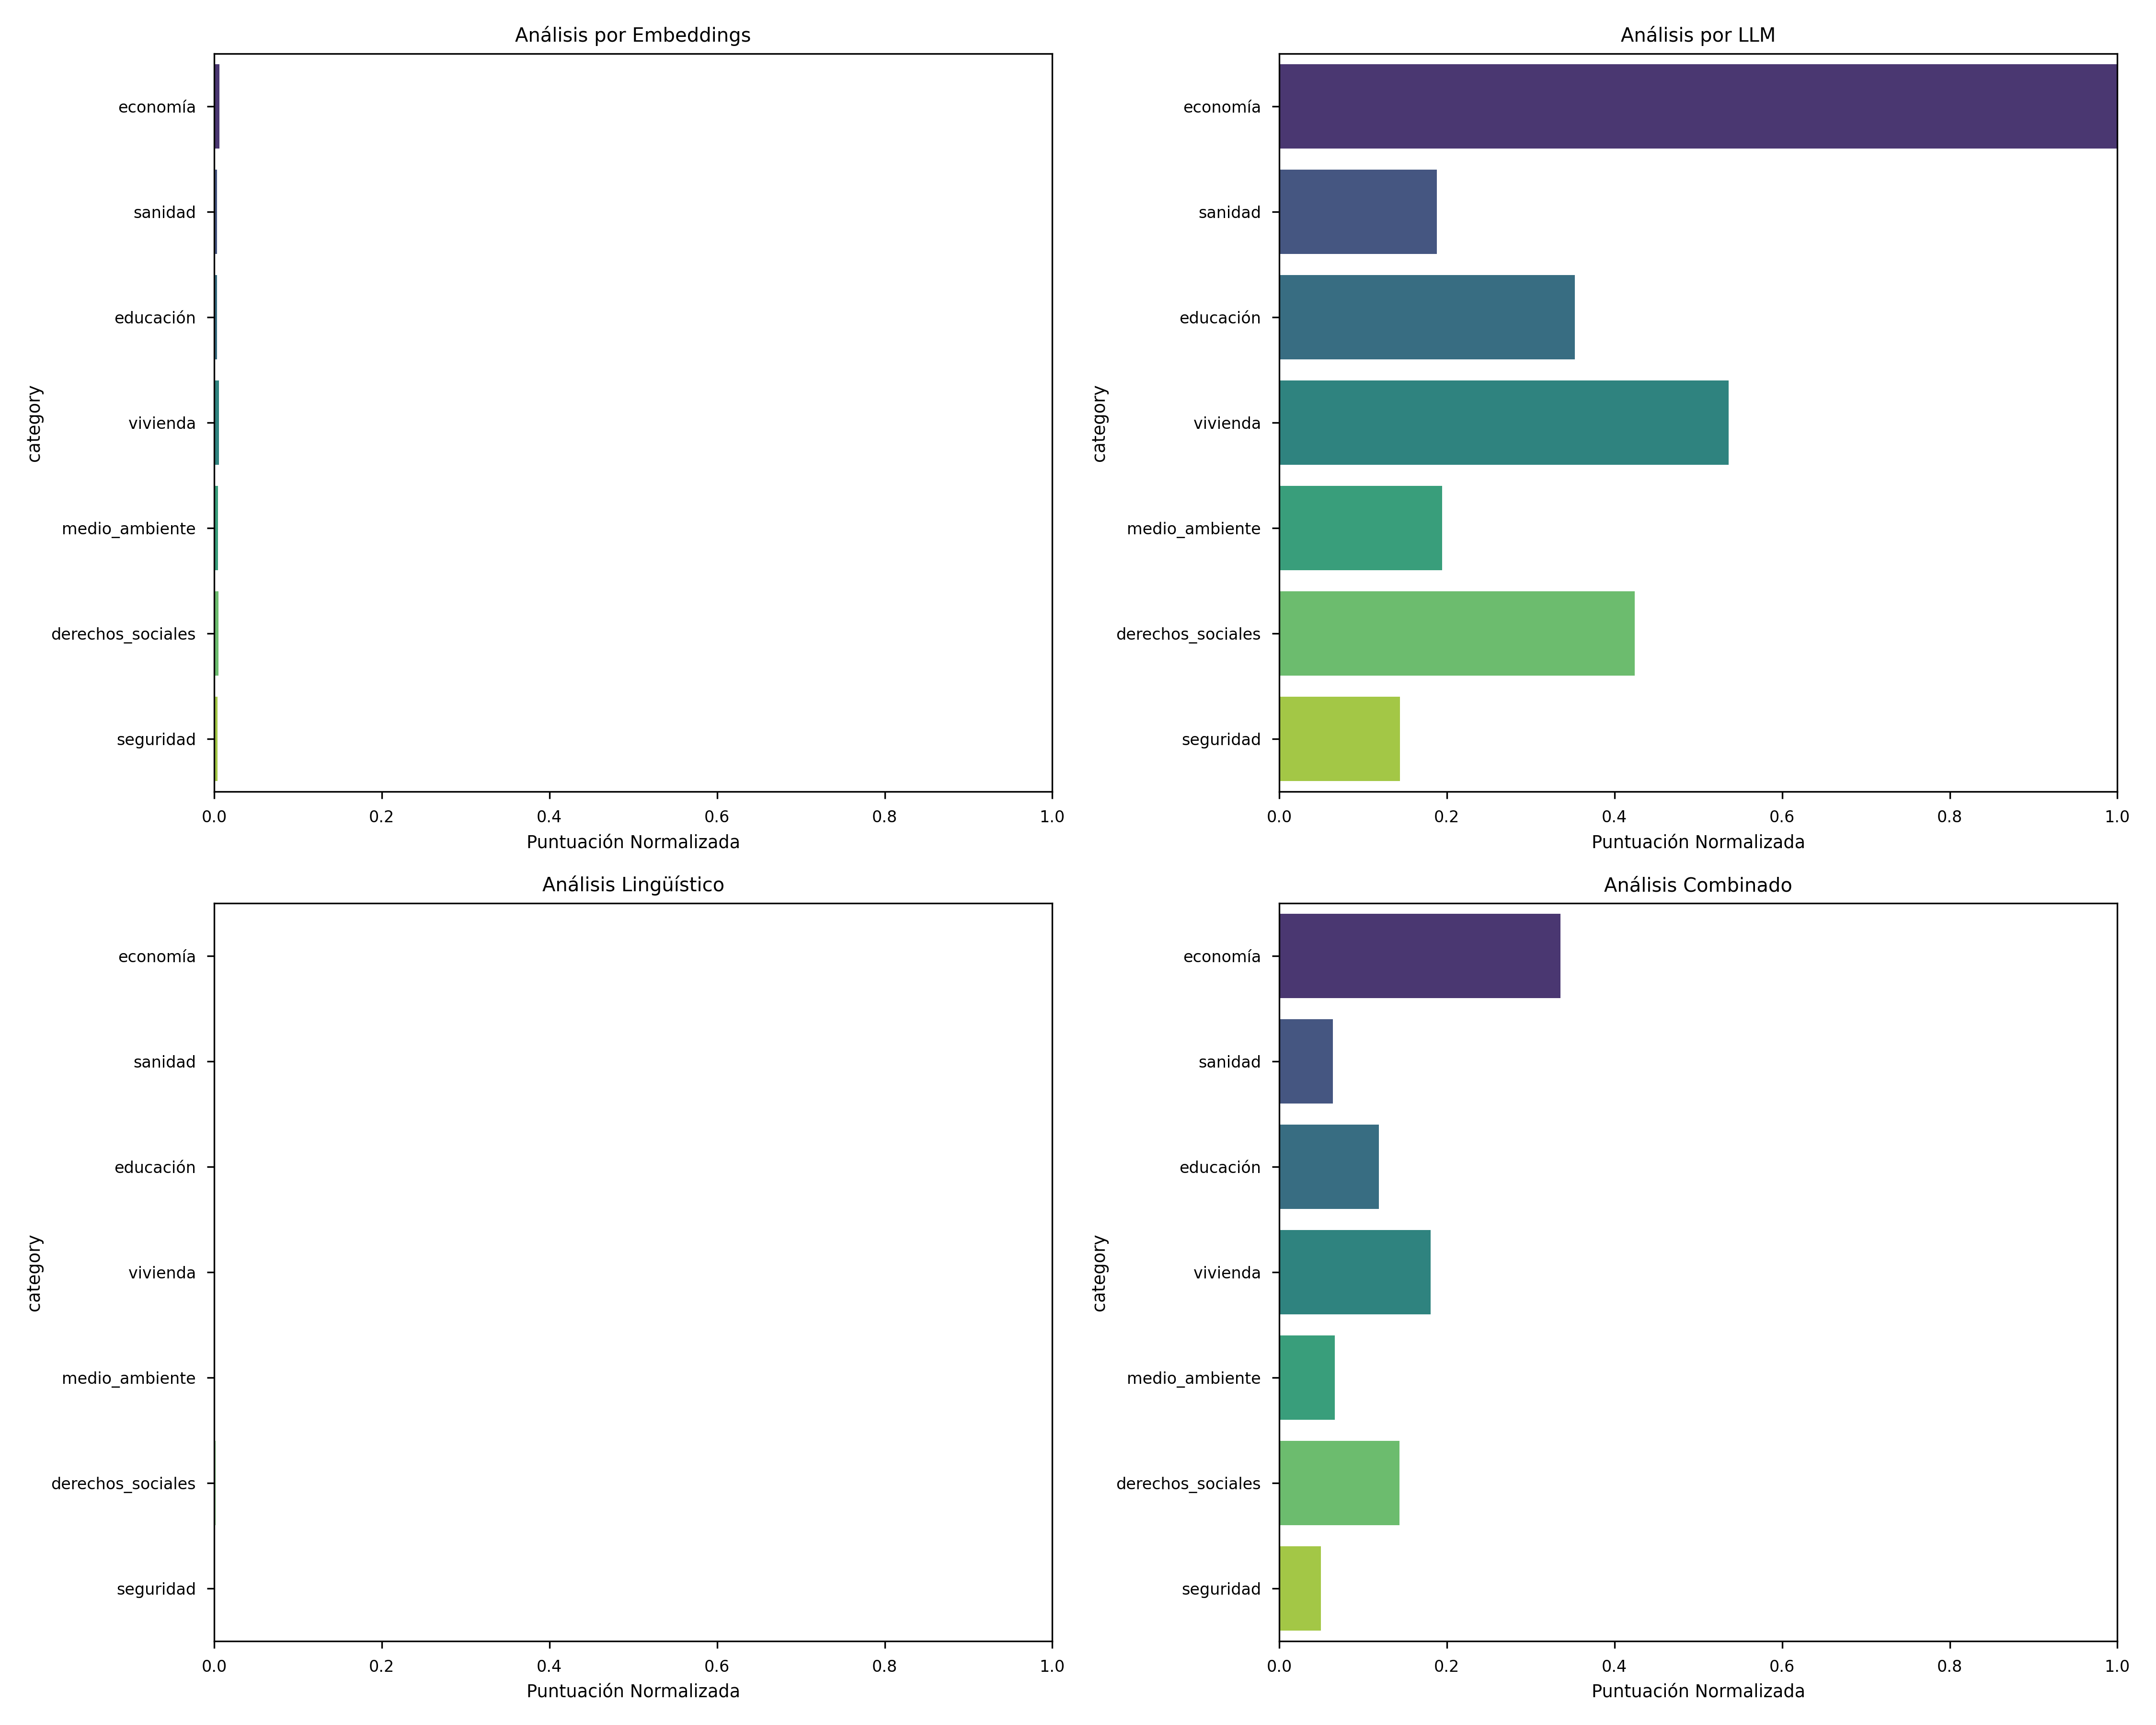
\includegraphics[width=0.8\textwidth]{ topic_distribution_by_method.png }
    \caption{ Distribución de Temas por Método }
    \label{fig:topic_distribution_by_method}
\end{figure}

\begin{figure}[H]
    \centering
    
\includegraphics[width=0.8\textwidth]{ topic_network.png }
    \caption{ Red de Relaciones entre Temas }
    \label{fig:topic_network}
\end{figure}


\end{document}